\subsection{Preventing traffic congestions for a one-lane road}\label{sec:traffic_congestion}

Traffic congestion, also known as traffic jams, is when a long line of vehicles moves slowly or has stopped moving altogether. Traffic jams can create frustration and disrupt nearby local environments with sound and gas emissions \parencite{traffic_congestion_pollution}. Many factors can cause traffic congestion, such as: poorly designed roads, not wide enough roads, traffic light patterns, and accidents \parencite{traffic_congestion}.

With this in mind, we started by focusing on a simple scenario: when a car drastically reduces its speed or completely stops on a single-lane road.

This scenario will lead to the vehicles behind needing to slow down drastically as well. This phenomenon is called traffic jam shockwave \parencite{traffic_shockwave}. To prevent this, we propose a solution where cars reduce their velocity before they reach the destination of where the shockwave started. For this to happen, a server could keep track of the cars' positions and send information to the vehicles behind, when required. 

We came up with an idea on how the server and cars should interact. First, the car would connect to the server and provide information about its current speed, weight, width, and length. The server will use this information to keep track of all the cars' positions on the road. The cars would send information to the server if their velocity changed. This message would trigger an event on the server where it would command all the cars behind to slow down accordingly. \figref{fig:diagramfirst} shows a flow chart of a potential simulation of this solution:

\begin{figure}[h!]
	\centering
	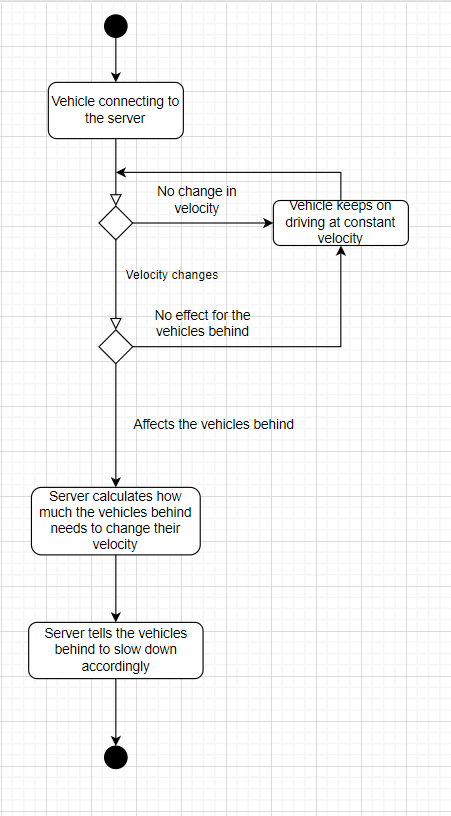
\includegraphics[width=0.9\linewidth]{figures/flow_diagram_first}
	\caption[Flow diagram server]{This figure shows the flow diagram of our first proposed solution. }
	\label{fig:diagramfirst}
\end{figure}